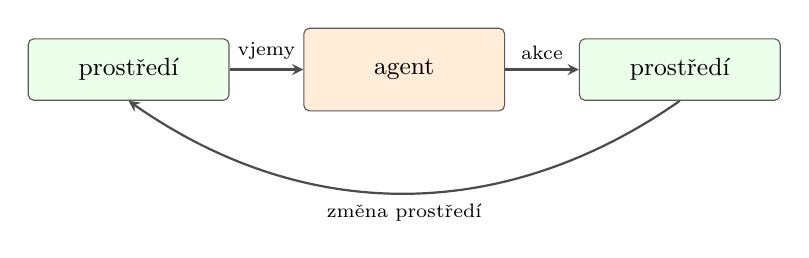
\begin{tikzpicture}[
    >=stealth,
    box/.style={
        draw=black!65,
        rounded corners=2pt,
        minimum width=2.55cm,
        minimum height=0.78cm,
        align=center,
        font=\small
    },
    env/.style={box, fill=green!8},
    agent/.style={box, fill=orange!15, minimum height=1.05cm},
    arr/.style={->, thick, draw=black!70}
]
    \node[env] (env1) at (-3.5,0) {prostředí};
    \node[agent] (agent) at (0,0) {agent};
    \node[env] (env2) at (3.5,0) {prostředí};

    \draw[arr] (env1) -- node[above, font=\scriptsize] {vjemy} (agent);
    \draw[arr] (agent) -- node[above, font=\scriptsize] {akce} (env2);

    \draw[arr, bend left=35] (env2.south) to node[below, font=\scriptsize] {změna prostředí} (env1.south);
\end{tikzpicture}
